\chapter{The dependency grammar}
\label{ch:dependecy-grappamr}

The Stanford dependency analysis of a given text constitutes the input for the algorithm developed in the current work. It provides the foundation to build the syntactic backbone used adopted here. This chapter offers an overview of the grammar and the parser developed at the Stanford university. In the last part of the chapter is discussed the cross theoretical connection between the dependency and systemic functional grammars. 

\section{An introduction to dependency theory of grammar}
%In this section I outline the theory of dependency grammar. I will make references sometimes to concepts in SFG. 
For the first time a complete linguistic theory based on the dependency concept was elaborated by the French linguist Lucien Tesniere in his seminal work \textit{``Elements de syntaxe strusturale''} published in \citeyear{Tesniere59} after his death. He devoted much effort to argue for the adequacy of \textit{dependency} as the organizational principle underlying numerous phenomena and in fact attempting to demonstrate the universality of his syntactic analysis method for human languages. In doing so he introduced a series of concepts and ideas among which the \textit{verb centrality}, \textit{stratification}, \textit{language typology}, \textit{nuclei}, \textit{valency}, \textit{metataxis}, \textit{junction} and \textit{transfer} are the most important ones which I introduce following the connections.

%His work, originally in French, has been translated in multiple languages German, Russina, Spanish, Japanese, Italian and recently in English \citep{Tesniere2015}.

\begin{quotation}
    The sentence is an \textit{organized set}, the constituent elements of which are the words. Each word in a sentence is not isolated as it is in the dictionary. The mind perceives \textit{connections} between a word and its neighbours. The totality of these connections forms the scaffold of the sentence. These connections are not indicated by anything. But it is absolutely crucial that they be perceived by the mind; without them the sentence would not be intelligible. \citep[3]{Tesniere2015}
\end{quotation}

Tesniere holds the view that the connection, what is know today as \textit{dependencies}, are the foundations of the \textit{structural syntax} known as \textit{dependency grammar} today. According to him ``to construct a sentence is to breathe life into an amorphous mass of words, establishing a set of connections between them. Conversely, understanding a sentence involves seizing upon the set of connections that unite the various words'' \citep[4]{Tesniere2015}. He introduces the hierarchy of connections as follows. 

\begin{quotation}
    Structural connections establish \textit{dependency} relations between words. In principle, each connection unites a superior term and an inferior term. The superior term is called the \textit{governor}, and the inferior term the \textit{subordinate}. We say that the subordinate depends on the governor and that the governor governs the subordinate. [\dots] A word can be both subordinate to a superior word and governor of an inferior word. [\dots] The set of words of a sentence constitutes a veritable \textit{hierarchy}. \citep[5--6]{Tesniere2015}
\end{quotation}

Introduction of hierarchy and governor-subordinate dependencies permeates definition \textit{node} and \textit{stemma} now known as \textit{dependency tree}. 

\begin{quotation}
    [\dots] In principle, a subordinate can only depend on a sole governor. A governor, in contrast, can govern multiple subordinates [...] Every governor that governs one or more subordinates forms what we call a node.  [\dots] it follows that \textit{each subordinate shares the fate of its governor}. \citep[6]{Tesniere2015}
\end{quotation}

\begin{figure}[!ht]
    \centering
    \begin{tikzpicture}
    \node[] (speaks) {speaks};
    \node[below=1em of speaks] (alfred) {Alfred};
    \draw[] (speaks) -- (alfred);
    \end{tikzpicture}
    \label{fig:stemma1}
    \caption{Stemma for ``Alfred speaks''}
\end{figure}

This asymmetry of connection permits construction of a tree-like structure. The diagram of the two word sentence ``Alfred speaks'' is provided in the Figure \ref{fig:stemma1}. The word \textit{speaks} is the governor of the word \textit{Alfred}. The connection is depicted bu the vertical line connecting the two. But to make it complete it is important to decide on the root node. 

\begin{quotation}
    The node formed by the governor that governs all the subordinates of a sentence is the \textit{node of nodes}, or the central node. It is at the center of the sentence and ensures its structural unity by tying the diverse elements into a single bundle. It can be identified with a sentence. \textit{The node of nodes is generally verbal} [\dots] \citep[7]{Tesniere2015}
\end{quotation}

% the verb centrality
The fundamental insight presented above about the nature of the syntactic structure concerns the grouping of words at the clause level. Tesniere rejects the subject-predicate formation that was the de facto syntactic understanding of his time. He argued that this division is belongs to Aristotelian logic and is not associated to linguistics. Instead of the subject-predicate division Tesniere positions the verb at the root of the clause structure making the subject and the object subordinated seedlings. Figure \ref{fig:stemma2} depicts the clause structure ``Alfred speaks slowly'' where both the subject and the object are subordinated to the central verb speaks. 

\begin{figure}[!ht]
    \centering
    \begin{tikzpicture}
    \node[] (speaks) {speaks};
    \node[below=1em of speaks, xshift=-2em] (alfred) {Alfred};
    \node[below=1em of speaks, xshift=2em] (slowly) {slowly};
    \draw[] (speaks) -- (alfred);
    \draw[] (speaks) -- (slowly);
    \end{tikzpicture}
    \label{fig:stemma2}
    \caption{Stemma for ``Alfred speaks slowly''}
\end{figure}

% stratification
Tesniere is among pioneer linguists recognising that the language is organised at different levels thus advocating a \textit{stratified model of language}. He recognises the to dimensional syntactic representation and the one dimensional chain of spoken language. 

\begin{quotation}
    \textit{speaking} a language involves transforming structural order to linear order, and conversely, \textit{understanding} a language involves transforming linear order to structural order. The fundamental principle of transforming structural order to linear order involves changing the connections of structural order into the sequences of linear order. This transformation occurs in such a manner that the elements connected in structural order become immediate neighbours in the spoken chain \citep[12]{Tesniere2015}.
\end{quotation}

% syntax semantix difference
In the structural realm Tesniere goes even deeper and describes the separation between syntax and semantics. To argue for that, he uses an example similar to the famous Chomskian ``Colourless green ideas sleep furiously'' \citep{Chomsky57} (that occurred three years after Tesniere's death). He employed the sentence ``The vertebral silence antagonizes the lawful sail''.

\begin{quotation}
    Syntax is distinct from morphology, and it is no less distinct from semantics. The structure of a sentence is one thing, and the idea that it expresses and that constitutes its meaning is another. It is therefore necessary to distinguish between the structural plane and the semantic plane.
    [\dots]
    The structural plane and the semantic plane are therefore entirely independent of each other from a theoretic point of view. The best proof is that a sentence can be ­semantically absurd and at the same time syntactically perfectly correct. \citep[33]{Tesniere2015}.
\end{quotation}

% nodes and nuclei
Tesniere distinguishes between \textit{nodes} and \textit{nuclei}. Initially he defines the node in a way that resembles the phrase or a constituent but after that he changes his mind.  

\begin{quotation}
    we define a \textit{node} as a set consisting of a governor and all of the subordinates that are directly or indirectly dependent on the governor and that the governor in a sense links together into a bundle. \citep[6]{Tesniere2015}.
\end{quotation}

Latter in the book, he uses the term node to mean merely a vertex and even redefines it saying that ``The node is nothing more than a geometric point whereas the nucleus is a collection of multiple points \dots'' \cite[39]{Tesniere2015}. It is perhaps the inconsistent use of the terminology that lead to the assumption that the dependency grammar does not recognises phrases (i.e. that is the complete subtree of a vertex). In fact he defines nucleus as playing the role of both a semantic and syntactic unit.

\begin{quotation}
    We define the nucleus as the set which joins together, in addition to the structural node itself, all the other elements for which the node is the structural support, starting with the semantic elements. \citep[38]{Tesniere2015}.
\end{quotation}

%valency
A notable contribution to the field of syntax is the concept of \textit{valency}. It is the notion used in other linguistic schools (e.g. \textit{transitivity}) to express combinatorial properties of verbs and other lexical items. Inspired from natural sciences, Tesniere compares the relationship between verbs and the so called \textit{actants} (known as \textit{arguments}) to atom's bonds. 

\begin{quotation}
    The verb may therefore be compared to a sort of atom, susceptible to attracting a greater or lesser number of actants, according to the number of bonds the verb has available to keep them as dependents. The number of bonds a verb has constitutes what we call the verb’s \textit{valency} \citep[241]{Tesniere2015}.
\end{quotation}

%He distinguishes \textit{avalent}, \textit{monovalent}, \textit{bivalent} and \textit{trivalent} verbs. 
Atoms are not the only metaphor he uses and next I present another one regarding the \textit{verbal node} that is especially important for showing the syntax-semantics interplay. 

\begin{quotation}
     The verbal node, found at the center of the majority of European languages, is a theatrical performance. Like a drama, it obligatorily involves a \textit{process} and most often \textit{actors} and \textit{circumstances}. [\dots] Transferred from the theatre to structural syntax, the process, the actors, and the circumstances become respectively the \textit{verb}, the \textit{actants}, and the \textit{circumstants} \citep[97]{Tesniere2015}.
\end{quotation}

Comparison of the verb to an atom seems to emphasize connection to the syntactic aspect of valency while comparing it to a theatrical performance seems to emphasize the semantic properties of valency. Therefore his theory of valency has semantic and syntactic properties. He believed that the first actant is the agent of the action, identified as the subject in traditional grammar, and the second actant is the one that bears the action, identified as the syntactic object. Tesniere regards both of them as complements to complete the governor verb making, in this sense, the subject indistinguishable from other complements. 

%junction
There are some problematic phenomena such as \textit{coordination} or \textit{apposition} because they are not governor-subordinate relations but are rather orthogonal relations among siblings. Tesniere analyses the coordination, or as he calls it \textit{junction}, as a phenomena used in language to express (semantic) content efficiently. 

He viewed the junction as fundamentally different from the subordination  and represented it with horizontal lines. Subordination is a principle of organization on the vertical axis whereas the coordination (i.e. junction) on the horizontal axis. Figure \ref{fig:stemma3} depicts two example representations for the sentence ``Young boys and girls played'' and ``Alfred adores cookies and detests punishments''. 

\begin{figure}[!ht]
    \centering
    \begin{subfigure}{.35\textwidth}
        \centering
        \begin{tikzpicture}
        \node[] (played) {played};
        \node[below=1em of played, xshift=-3em] (boys) {boys};
        \node[below=1em of played, xshift=0em] (and) {and};
        \node[below=1em of played, xshift=3em] (girls) {girls};
        \node[below=4em of played, xshift=0em] (young) {young};
        \draw[] (played) -- (boys);
        \draw[] (played) -- (girls);
        \draw[] (and) -- (girls);
        \draw[] (and) -- (boys);    
        \draw[] (young) -- (boys);
        \draw[] (young) -- (girls);
        \end{tikzpicture}
        \caption{Young boys and girls played}
        \label{fig:stemma3-sub1}
    \end{subfigure}%
    \begin{subfigure}{.65\textwidth}
        \centering
        \begin{tikzpicture}
        \node[] (adores) {adores};
        \node[right=1em of adores] (and) {and};
        \node[right=1em of and] (detests) {detests};
        \node[below=4em of adores, xshift=-3em] (alfred) {Alfred};
        \node[below=4em of adores, xshift=3em] (cookies) {cookies};
        \node[below=4em of detests, xshift=0em] (pun) {punishments};
        \draw[] (adores) -- (alfred);
        \draw[] (adores) -- (cookies);
        \draw[] (and) -- (adores);
        \draw[] (and) -- (detests);    
        \draw[] (detests) -- (pun);
        \end{tikzpicture}
        \caption{Alfred adores cookies and detests punishments}
        \label{fig:stemma3-sub2}
    \end{subfigure}
    \caption{Sample stemmas with \textit{junction} representation}
    \label{fig:stemma3}
\end{figure}

%The junction is total when the conjuncts shared their heads and/or dependents and partial when some are not shared. For the total junction Tesniere used terms of heraldry: \textit{coped} (upwards triangle formed by two conjuncts sharing a dependant), \textit{shod} (downwards triangle formed by a head governing two conjuncts) and \textit{dressed} (diamond formed by conjuncts with one shared head and one shared dependant). The partial structures are called \textit{bifid} are asymmetric one way or another and are classified as \textit{anadidymic}, \textit{catadidymic}, \textit{anacatadidymic}

%transfer
A big part of the Tesniere's \textit{Elements} \citep{Tesniere59} is dedicated to the theory of \textit{transfer}. It describes the phenomena when one class of a syntactic unit occupies a position usually devoted to another one. For example the noun can be transferred to an adjective by preposition ``of'', as for example \textit{a linguist of France} where the source \textit{France} is transferred to target \textit{of France} which modify \textit{linguist} that is typically an adjectival function. Transfer is a tool that explains how for example a clause can be embedded into another one or how a verb can be subordinate to another one. 

Tesniere splits the words into \textit{function words} or \textit{translatives} (i.e. prepositions, conjunctions, auxiliary verbs and articles) and four basic categories of \textit{content words} (i.e. verbs (I), nouns (O), adverbs (E) and adjectives (A) ). The former are empty of content marker transfer of content words from one syntactic category to another one. That is, allowing one word to occupy a position that is generally associated with a word of another category. 

One distinguishing trait of the transfer is that the words transferred from source to target category continue to behave as the source category with respect to their dependants and as source category to its governor.

The transfer theory is controversial for the translators of the Elements. They write \citep[liv-lx]{Tesniere2015} that while the transfer schema can not be interpreted in terms of pure dependency it is debatable whether it can be interpreted in terms of constituency. The main distinction is in the number of nodes that one assumes to be in the syntactic structure i.e. whether there are intermediary virtual nodes. 

\begin{figure}[!ht]
    \centering
    \begin{subfigure}{.33\textwidth}
        \centering
        \begin{tikzpicture}
        \node[] (XP) {XP};
        \node[below=1em of XP, xshift=-2em] (X) {X};
        \node[below=1em of XP, xshift=2em] (Y) {Y};
        \draw[] (XP) -- (X);
        \draw[] (XP) -- (Y);
        \end{tikzpicture}
        \caption{Headed endocentric}
        \label{fig:stemma4-sub1}
    \end{subfigure}%
    \begin{subfigure}{.33\textwidth}
        \centering
         \begin{tikzpicture}
        \node[] (YP) {YP};
        \node[below=1em of YP, xshift=-2em] (X) {X};
        \node[below=1em of YP, xshift=2em] (Y) {Y};
        \draw[] (YP) -- (X);
        \draw[] (YP) -- (Y);
        \end{tikzpicture}
        \caption{Headed endocentric}
        \label{fig:stemma4-sub2}
    \end{subfigure}
    \begin{subfigure}{.33\textwidth}
        \centering
     \begin{tikzpicture}
        \node[] (XP) {ZP};
        \node[below=1em of XP, xshift=-2em] (X) {X};
        \node[below=1em of XP, xshift=2em] (Y) {Y};
        \draw[] (XP) -- (X);
        \draw[] (XP) -- (Y);
    \end{tikzpicture}
    \caption{Non-headed exocentric}
    \label{fig:stemma4-sub3}    
    \end{subfigure}
    \caption{Constituency structure}
    \label{fig:stemma4}
\end{figure}

\begin{figure}[!ht]
    \centering
    \begin{subfigure}{.33\textwidth}
        \centering
        \begin{tikzpicture}
        \node[] (X) {X};
        \node[below=1em of X, xshift=2em] (Y) {Y};
        \draw[] (X) -- (Y);
        \end{tikzpicture}
        \caption{Headed endocentric}
        \label{fig:stemma5-sub1}
    \end{subfigure}%
    \begin{subfigure}{.33\textwidth}
        \centering
        \begin{tikzpicture}
        \node[] (X) {Y};
        \node[below=1em of X, xshift=-2em] (Y) {X};
        \draw[] (X) -- (Y);
        \end{tikzpicture}
        \caption{Headed endocentric}
        \label{fig:stemma5-sub2}
    \end{subfigure}
    \begin{subfigure}{.33\textwidth}
        \centering
        \begin{tikzpicture}
        \node[] (XP) {$\emptyset$};
        \node[below=1.2em of XP, xshift=-2em] (Y) { };
        \end{tikzpicture}
        \caption{Non-headed exocentric}
        \label{fig:stemma5-sub3}
    \end{subfigure}
    \caption{Dependency structure}
    \label{fig:stemma5}
\end{figure}


Figure \ref{fig:stemma4} shows how a sequence of two elements X and Y can be represented in terms of constituency where the Figure \ref{fig:stemma4-sub1} and \ref{fig:stemma4-sub2} represent that one element governs the other called \textit{endocentric} structures and in Figure \ref{fig:stemma4-sub3} a non-headed structure called \textit{exocentric}. Dependency structure depicted below in Figure \ref{fig:stemma5}, in contrast, cannot represent non-headed structures. Hence there is no correspondent dependency representation to Figure \ref{fig:stemma4-sub3} in Figure \ref{fig:stemma5-sub3}. 

Bringing back the discussion on the number of nodes, the constituency structure requires three nodes each time whereas dependency structure only two. In this sense the transfer schemas provided by Tesniere in his Elements \citep{Tesniere59} resembles constituency structure more than dependency structure simply because it assumes more nodes than words. 

%TODO compare transformation to the gramatical metaphor, see the definitiopn of the grammatical metaphor https://www.thoughtco.com/grammatical-metaphor-or-gm-1690913
%Elements - transaltors ppt - http://depling.org/depling2015/Tesniere.pdf
%Elements - transaltors intro - https://kahanedotfr.files.wordpress.com/2017/01/tesniere-introduction-benjamins2015.pdf



%
%
%



Traditionally, Latin language tended to be analysed with the \textit{dependency model} based on theories of what was called \textit{government}. It explains the syntagmatic relations of the subtype Firth called \textit{colligation} (i.e. relations between grammatical categories). Government is a way of explaining the rich inflections of language (such as Latin) in terms of how particular words govern, that is to say, determine, the inflection of other words. \citep[p.66]{McDonald2008}

\citet{Tesniere2015} explains how government works by giving example of Latin text analysis where the inflections immediately give aloto of information about relations between different words. For example the verb agree in person and number with its subject. From this point of view the verb governs the subject. The verb also governs complements and adjuncts which can be seen as relations of dependency between a governing element or controller and a governed element or dependant. It is important to note that Tesniere analysed syntax at the level of clause where he identified a verb node as the main controller. 

Contrary to Latin, languages like English or Chinese, where there is little or most of the time none of the inflectional marking to identify dependency relations, are much harder to analyse in terms of such relations. This was a motivation for Tesniere to reinterpret dependency relation in semantic terms rather than inflectional marking. As \citet{McDonald2008} points out, this can be regarded as extending syntagmatic relations of the clause to include what Firth was calling \textit{collocation} relations (i.e. links between lexical items). Tesniere framed his theory in terms of syntagmatic relations as expressing a model of experience. He compares the verbal node of the clause to a complete little drama. Like a drama, it obligatorily consists of an action, most often actors and features of settings. Expressed in terms of syntactic structure, the action, actors and settings become the verb, participants and circumstances \citep{Tesniere2015}. 

Further, Tesniere explains \textit{categories of language} as \textit{categories of thought}. The human mind shapes the world in its own measure by organising experience into a systematic framework of ideas and beliefs called categories of though. Likewise, the language shapes thought in its own measure by organising it into a systematic framework of grammatical categories \citep{Tesniere2015}. He stresses though, that the latter ones can vary considerably from language to language and that the analysis of syntactic relations shall be carried on not in terms of grammatical categories but rather in terms of functions. He explain through an example that analysis in terms of nouns and verbs i.e. grammatical categories, tells nothing about the tie that links the words, whereas if we turn to notions such as subject and complement it all of the sudden becomes clear: the connections are established, the lifeless words become a living organism and the sentence take on a meaning \citep{Tesniere2015}.

\section{Stanford dependency grammar (and parser)}
Dominant \citet{Chomsky1981} theories define grammatical relations as configurations of \textit{phrase structure} representations, which is nesting of multi word constituents. Other theories such as Lexical-Functional Grammar reject the adequacy of such an approach \citep{Brensan2000} and advocate a functional representation for syntax.

When motivating its stance, \citet{Marneffe2006} insists on practical rather than theoretical concerns proposing that structural configurations be defined as grammatical roles (to be read as grammatical functions)\citep{Marneffe2006}. For example she insists that, information about functional dependencies between words grants direct access to the predicate-argument relations which are not readily available form the phrase structure parses and can be used off the shelf for real world applications. She avoids going into theoretical debates and focuses on the suitability of the grammar for parsing within the context of relation extraction, machine translation, question answering and other tasks.

The functional dependency descriptions is precisely the aspect which makes possible the link between the Stanford Dependency Grammar and Systemic Functional Structures targeted in the current thesis. 

%\section{The dependency set}
The design of Stanford dependency set \citep{Marneffe2006, Marneffe2008,  Marneffe2014, Silveira2014} bears a strong intellectual debt to the framework of Lexical Functional Grammars \citep{Brensan2000}. \citet{Marneffe2006} started designing the relation typology from GR \citep{Carroll1999} and PARK \citep{King2003} schemes following a LFG style and according to the principles described in Generalization \ref{def:design-principles}.

\begin{generalization}[Design principles for Stanford dependency set]\label{def:design-principles}\leavevmode
	\begin{enumerate}
		\item Everything is represented uniformly and some binary relation between two sentence words.
		\item Relations should be semantically contentful and useful to applications.
		\item Where possible, relations should use notions of traditional grammar \citep{Quirk1985} for easier comprehension by users.
		\item The representation should be spartan rather than overwhelming with linguistic details. 
	\end{enumerate}
\end{generalization}

When proposing the Stanford dependency, \citet{Marneffe2006} inherits many relations from Lexical Functional Grammars\citep{Brensan2000} and departs from the sets described by \citet{Carroll1999} and \citet{King2003}. She arranges the grammatical relations into a hierarchy rooted in a generic relation \textit{dependent}. This is then classified into a more fine-grained set of relations between a head and its dependent. 
%TODO continue describing Stanford dependecy set 

\section{Stanford Parser: collapsed-cc output}
\label{sec:collapsed-cc-output}
% describing the cc-collapsed
The Stanford Dependency Parser is capable of generating several types of dependency representations. The most convenient and informative version is Collapsed-CC-processed. This structure is created after the initial parse is ready and constitutes a simplified and more intuitive representation of the dependency parse. The collapsed form concerns prepositions, conjunctions and relative clause referents. Dependencies involving prepositions and conjunctions are transformed from basic form in Figure \ref{fig:prep-transf1} to the form where preposition are embedded into the edge relation, as in Figure \ref{fig:prep-transf2}. Similar transformation is done for conjunctions. 

\begin{figure}
	\centering
	\begin{minipage}[b]{0.45\textwidth}
		\centering
		\begin{dependency}[dep-style]
			\begin{deptext}[]
				based \& in \& Luxembourg\\
			\end{deptext}
			\depedge{1}{2}{prep}
			\depedge{2}{3}{pobj}
		\end{dependency}
		\caption{Basic(uncollapsed) preposition dependency}
		\label{fig:prep-transf1}
	\end{minipage}
	\quad
	\begin{minipage}[b]{0.45\textwidth}
		\centering
		\begin{dependency}[dep-style]
			\begin{deptext}[]
				based \& in \& Luxembourg\\
			\end{deptext}
			\depedge{1}{3}{prep\_in}
		\end{dependency}
		\caption{Collapsed preposition dependency}
		\label{fig:prep-transf2}
	\end{minipage}
\end{figure}

Besides collapsing prepositions and conjunctions the DG is further processed to introduce more relations (i.e. connections) even if they break the tree structure. For example the \textit{ref} relation does not appear in the basic dependency structure in figure \ref{fig:rel-transf1} but it appears in the processed dependency structure forming a cycle with \textit{rcmod} and \textit{subjpass} relations.

\begin{figure}
	\centering
	\begin{minipage}[b]{0.45\textwidth}
		
		\begin{dependency}[dep-style-narrow]
			\begin{deptext}[]
				Nina \& , \& who \& is \& coming \& tomorrow\\ % \& , \& makes \& ... \\
			\end{deptext}
			\depedge[edge unit distance =2.2ex]{1}{5}{rcmod}
			\depedge{5}{3}{nsubjpass}
			\depedge{5}{4}{auxpass}
			\depedge{5}{6}{tmod}
		\end{dependency}
		\caption{Basic(uncollapsed) preposition dependency}
		\label{fig:rel-transf1}
	\end{minipage}
	\quad
	\begin{minipage}[b]{0.45\textwidth}
		\centering
		\begin{dependency}[dep-style-narrow]
			\begin{deptext}[]
				Nina \& , \& who \& is \& coming \& tomorrow\\ % \& , \& makes \& ... \\
			\end{deptext}
			\depedge[edge unit distance =2.2ex]{1}{5}{rcmod}
			\depedge{1}{3}{ref}
			\depedge{5}{3}{nsubjpass}
			\depedge{5}{4}{auxpass}
			\depedge{5}{6}{tmod}
		\end{dependency}
		\caption{Collapsed preposition dependency}
		\label{fig:rel-transf2}
	\end{minipage}
\end{figure}

Relations like \textit{ref} introduce cycles but add valuable information useful in various stages of further processing. However, ensuring a tree structure in important for the CG creation stage because it is based on a top down traversal. This is taken care of in the preprocessing stage described in the next stage.

\section{Penn part-of-speech tag set}
%NOTE: this section is transfered into SFL grammar chapter
%In traditional grammar \textit{word classes} or \textit{parts of speech} are a commonly accepted concept. However in SFL, it plays rather an orientation or an approximation role, precisely because the part of speech do not have one to one correspondence to the elements they expound. So terms such as \textit{noun} or \textit{adjective} are useful to denote a class of words that expound a certain element of the structure, but such word class to element correspondences shall by no means treated as definite rules. 
%This is in fact the approach taken in current work and correspondence mappings had between established between part of speech to the set of elements they may expound in various units. %TODO[JB] give examples

Stanford dependency parser starts creation of the parse structure process from the list of tokens annotated with Penn part-op-speech tags. Embedded into the dependency graph, these tags are the part of the syntactic context from which SFG constituency graph is built. 



\section{Cross theoretical bridge from DG to SFL}
\label{sec:cross-theoretical-bridge}
\label{sec:dependecy-relations-sfl}

The concept of dependency between pairs of words is long acknowledged in linguistic communities. In traditional terms dependencies are treated as \textit{hypotactic expansions} (see Definition \ref{def:taxis}) of word classes (or parts of speech) where the expanded word acts as \textit{heads} and expanding ones as \textit{dependent} establishing parent-daughter structural relations illustrated in Figure \ref{fig:dependecy-dg}.
%and the description of \citet[pp. 438 -- 443]{Halliday2013}


%\todo{Next I will describe an example of two structures side by side and show how correspondences between the two can be established.}
%\subsection{The nature of dependency}

% head modifier discussion
%\todo{review, new title, talk about , present comparison between parent-daughter and orthogonal/sister dependecy within constituents}

In SFL community the concept of dependency is less salient than the foundational role it plays in the Dependency Grammars. Dependencies are regarded as orthogonal relations between sibling elements of a unit (Figure \ref{fig:dependecy-sfg}) and link the \textit{heads} to their \textit{modifies} in by Hallidayan \textit{logical structure}\citep{Halliday2013}. 

%Within dependency structure the relation is defined as \textit{parent-daughter dependency} while SFL constituency structure the relation is of \textit{sibling dependency}. 

Figure \ref{fig:dependency-relations} illustrates side by side the parent-daughter and sibling dependency relations. In Figure \ref{fig:dependecy-dg} dependency are the only relations between the units of structure whereas in Figure \ref{fig:dependecy-sfg} there are multiple levels (ranks) of units and the dependency relations are relevant only between siblings at the same level within the structure of an unit. SFL regards dependency relations holding only between elements of a unit whereas the relations that connect the units of lower and higher rank are \textit{constituency relations}. Yet when we look at the two structures they resemble in a way each other and next I show how. 

\begin{figure}[hbtp]
	\centering
	\begin{subfigure}{.5\textwidth}
		\centering
		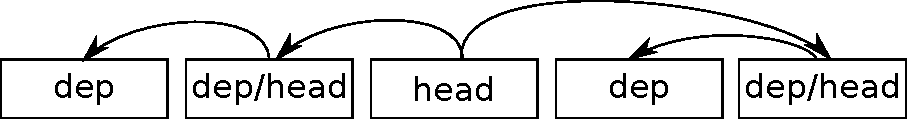
\includegraphics[width=0.9\textwidth]{Figures/SFL-grammar/dependency-dg.pdf}
		\vspace{+22pt}
		\caption{The parent-daughter relations in DG}
		\label{fig:dependecy-dg}
	\end{subfigure}%
	\begin{subfigure}{.5\textwidth}
		\centering
		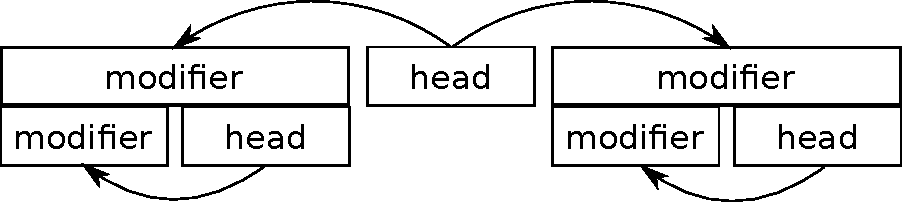
\includegraphics[width=0.9\textwidth]{Figures/SFL-grammar/dependency-sfg.pdf}
		\caption{The head-modifier relations in SFG}
		\label{fig:dependecy-sfg}
	\end{subfigure}
	\caption{The dependency relations in DG and SFG}
	\label{fig:dependency-relations}
\end{figure}

In a nutshell, the parent-daughter dependency relations in dependency grammar unpack into multiple function in systemic functional grammar and specifically it is the head-modifier indirect relation, unit-element componence relation and the head of unit a ``representativeness'' function. 

This difference implies that, when translated to a constituency unit (described in Section \ref{sec:creation-constituency-graph}), the dependency unit, stands for both a unit and that unit's head element. In other words a DG node corresponds to two functional elements at different rank scales. For example the root verb in dependency graph corresponds to the clause node and the lexical item which fills the Main Verb of the clause. By analogy, the head noun of a Nominal Group anchors the entire unit (as a group) and fills the head element of the group. 

\begin{table}[ht]
	\centering
	\begin{tabular}{|l|c|c|ccc}
		\hline
		\textbf{text}              & \textbf{some}                            & \textbf{very}                     & \multicolumn{1}{c|}{\textbf{small}} & \multicolumn{1}{c|}{\textbf{wooden}}            & \multicolumn{1}{c|}{\textbf{ones}}          \\ \hline
		\textbf{units}    & \multicolumn{5}{c|}{\textbf{Nominal Group}}                                                                                                                           \\ \hline
		\textit{elements} & \textit{Quantifying Determiner} & \multicolumn{2}{c|}{\textit{Modifier}}                & \multicolumn{1}{c|}{\textit{Modifier}} & \multicolumn{1}{c|}{\textit{Head}} \\ \hline
		\textbf{units}    &                                 & \multicolumn{2}{c|}{\textbf{Quality Group}}           & \multicolumn{2}{c}{\multirow{2}{*}{}}                                       \\ \cline{1-1} \cline{3-4}
		\textit{elements} &                                 & \textit{Degree Tamperer} & \textit{Apex}              & \multicolumn{2}{c}{}                   \\ \cline{1-1} \cline{3-4}
	\end{tabular}
	
	
	\caption{SF analysis of Example \ref{ex:small-wooden} (reproduced from Table \ref{tab:example-substructure-analisys-cardiff} )}
	\label{tab:example-substructure-analisys-cardiff-repeated}
\end{table}

\begin{figure}[ht]
	\centering
	\begin{dependency}[dep-style-narrow]
		\begin{deptext}[]
			some/DT \& very/RB \& small/JJ \& wooden/JJ \& ones/NNS \\
		\end{deptext}
		\depedge[edge unit distance =2.2ex]{5}{1}{det}
		\depedge{3}{2}{advmod}
		\depedge{5}{3}{amod}
		\depedge{5}{4}{amod}
	\end{dependency}
	\caption{Dependency analysis for Table \ref{tab:example-substructure-analisys-cardiff-repeated} }
	\label{fig:small-wooden-dependecy}
\end{figure}

%The dependency structure is overloaded with two kinds of meaning


Figure \ref{fig:small-wooden-dependecy} and the Table \ref{tab:example-substructure-analisys-cardiff-repeated} represent the analysis of a nominal group from Example \ref{ex:small-wooden} (``some small very small wooden ones'') in Cardiff grammar and Stanford dependency grammar exhibiting a contrast of the two structures. Consider the dependency relation ``det'' a link between the noun ``ones'' and the determiner ``some''. When translated into SF variant the dependency relation stands within Nominal Group between the Head element (filled by word ``ones'') and the Quantifying Determiner element (filled by the word ``some''). By definition all elements in a unit are equal in the structure so the Head and Quantifying Determiner are siblings. So the items (words) filling those elements are sibling. How is then the dependency relation established? 

In SFL there is the concept of Head and Modifier. There is no direct relationship between them but it is said that what the Modifier modifies is the Head. The relation is not a direct one, the Modifier and Head stand for two different kinds of meaning and what the Modifier modifies is not the Head per se but the referent denoted by the head (and thus construed by the entire unit). It is precisely this modification of the head that is called a (sibling) dependency relation and is seldom mentioned in SFL literature because it is considered implicit and recoverable from the SF constituency structure.

The Head also is the element that anchors the entire unit and plays a constitutive role. In this sense the word ``ones'' realizes not only the Head function (sided with Determiner ``some'') but also anchors the entire unit. The relation between the group and it's elements is one of \textit{componence} (Definition \ref{def:componence}) described in Section \ref{sec:componence}. Yet in the role of unit anchor we cannot say that there is a componence relation between ``one'' and ``some'' because it is merely a proxy to the referent rather than the entire unit. So in this role ``one'' can be said to be standing in a parent-daughter dependency relation to ``some'' incorporating the filling and componence relations.

I just showed how the dependency relation in dependency structure (Figure \ref{fig:dependecy-dg}) can be unpacked into two relations in systemic functional structure (Figure \ref{fig:dependecy-sfg}): sibling dependency considered an indirect relation between Head and Modifier (Logical Metafunction) and parent-daughter dependency between unit anchor and the compounding elements, relation which resembles unit componence but is not. 

Lets look at a second example of two relations ``advmod'' from ``small'' to ``very'' and ``amod'' from ``ones'' to ``small''. The interesting case here is the item ``small'' which is the Head of the Quality Group, it anchors the meaning of the whole group and the Quality group fills the Modifier element within the Nominal group. What is not covered in previous example is that the Apex ``small'' not only is a representative of the entire group but it also is a \textit{representative filler} of the Modifier element within Nominal Group. Using the similar translation mechanism as above, this means that, the incoming dependency needs to be unpacked into three levels: the element within the current group (Modifier), the unit class that element is filling (Quality Group) and finally the head of the filler group (Apex). In fact, to be absolutely correct there is one more level. The elements of a unit are expounded by lexical items, so fourth relation to unpack is the expounding of the Apex by ``small'' word.

In this section I laid the theoretical principle for transforming the dependency structure into systemic functional structure. In practice to achieve this level of unpacking the algorithm requires a bottom up and a top down contextualization in terms of elements of structure within a unit and realised sequence of textual units. This implied that the unpacking needs two traversals, a bottom-up and a top one. More on that and the exact algorithm for the translation is provided in Section \ref{sec:creation-constituency-graph}.

Next follows the chapter on Governance and Binding Theory needed to account for the unrealised, covert (Null) Elements in the syntactic structure. It is also an opportunity to perform a similar theoretical translation exercise (as in this section) from one theory of grammar into another.

%
%\todo{close the chapter}
%
%\explain{the problem of bottom up and top down view on the tree structure, due to the fact that head elements plays two roles: of the unit-class(from above) and head-element(from below)}
%\explain{how it is solved with two traversals in the syntactic parsing chapter}
%
%\section{Discussion}